\chapter[Dashboard, Deployment and Decision Support]{Business Intelligence Dashboard,\\ Deployment and Decision Support}\label{ch:dashboard}

\section{Design goals}
The dashboard is where the framework meets its users, the sales, supply-chain and senior managers. Following
\citet{few2013}, \citet{tufte2001} and \citet{knaflic2015}, it was designed to meet five requirements:
\begin{enumerate}
  \item \textbf{At-a-glance KPIs}: net sales, units, orders, average order value, discount rate and
        year-to-date growth appear at the top of the overview page;
  \item \textbf{Consistent filtering}: one set of filters (years, region, channel, customer type, category)
        applies across all pages;
  \item \textbf{The three management questions}: pages progress from \emph{what happened} (overview, trends,
        products, markets) to \emph{why} (drivers, segments) and \emph{what next} (forecast, anomalies,
        recommendations);
  \item \textbf{Honest presentation}: forecasts are always shown with prediction intervals, model accuracy is
        visible to users, and colour is used only to encode meaning. Following \citet{tufte2001}, decoration
        that carries no data (3-D effects, gauges, heavy grid lines) is avoided;
  \item \textbf{Free and accessible}: the dashboard runs in any web browser and is hosted at no cost.
\end{enumerate}

\section{Implementation}
The dashboard was built with Streamlit and Plotly in a single Python file (\path{dashboard/app.py}). It does
not read the 500,000 raw rows. It reads compact aggregates produced by the pipeline: a monthly cube by region
$\times$ channel $\times$ customer type $\times$ category, monthly product-by-region totals, forecasts, model
scores, segment tables and anomaly lists. Their total size is about 2~MB, so the application starts in seconds
on the free hosting tier, while every filter combination remains exact. Data are cached in memory after the
first load. Each page has its own web address (for example \path{?page=forecast}), so a manager can bookmark
or share a specific view. \Cref{tab:pages} lists the nine pages, and
\cref{fig:dashoverview,fig:dashtrends,fig:dashproducts,fig:dashmarkets,fig:dashforecast,fig:dashmodels,fig:dashanomalies,fig:dashinsights,fig:dashquality}
show each of them as deployed. All screenshots were captured automatically from the running application by
\path{tools/capture_screenshots.py}, so they can be refreshed whenever the data change.

\begin{table}[htbp]\centering\small
\caption{Pages of the interactive dashboard}\label{tab:pages}
\begin{tabularx}{\linewidth}{@{}lX@{}}
\toprule
\textbf{Page} & \textbf{Content} \\ \midrule
Executive overview & KPI cards, monthly sales with moving average, category, region and channel mix, annual table \\
Trends \& seasonality & Stacked trends by any dimension, year $\times$ month heat map, seasonal index, year-on-year lines \\
Products \& portfolio & Top-$N$ products, Pareto/ABC analysis, ML product segments, single-product drill-down \\
Markets \& customers & Region $\times$ channel heat maps, customer types, regional CAGR, ML market segments \\
Demand forecast & 12-month outlook with interval, category and product forecasts, model leaderboard, CSV download \\
Machine-learning models & Regression, classification and clustering results with feature importance \\
Anomaly monitor & Daily sales against expected level with flagged days; most suspicious orders \\
Insights \& recommendations & Automatically generated insights with recommended actions \\
Data quality \& method & Validation report, cleaning log and architecture diagram \\ \bottomrule
\end{tabularx}
\end{table}

\section{Walk-through of the dashboard}
\paragraph{What happened.} The \emph{executive overview} (\cref{fig:dashoverview}) opens with six KPI cards and
the monthly sales trend with its 12-month average. Below them, the category, region and channel mix and an
annual summary table answer the first questions a manager asks. The \emph{trends} page
(\cref{fig:dashtrends}) shows how any dimension develops over time and makes the December peak and February
trough visible in a year~$\times$~month heat map. The \emph{products} page (\cref{fig:dashproducts}) ranks the
products, draws the Pareto curve with ABC classes and lets the user drill down into a single product. The
\emph{markets} page (\cref{fig:dashmarkets}) compares regions, channels and customer types and shows the
market segments found by clustering.

\paragraph{What next.} The \emph{demand forecast} page (\cref{fig:dashforecast}) presents the 12-month outlook
with its 80\% prediction interval, forecasts by category and product, and the leaderboard of forecasting
models. The forecasts can be downloaded as CSV for the production plan. The \emph{machine-learning} page
(\cref{fig:dashmodels}) exposes the evidence behind the forecasts: test errors of all models against the
baselines, the recursive multi-step test and feature importance, plus the classification and clustering
results in separate tabs.

\paragraph{Control and action.} The \emph{anomaly monitor} (\cref{fig:dashanomalies}) plots daily sales against
the expected level, marks the flagged days and lists the most suspicious orders for checking. The
\emph{insights} page (\cref{fig:dashinsights}) turns all results into plain-language findings, each followed by
a recommended action. Finally, the \emph{data quality} page (\cref{fig:dashquality}) documents the validation
checks and the cleaning log, so users can see why the numbers can be trusted.

\newcommand{\dashshot}[3]{%
\begin{figure}[p]\centering
\includegraphics[width=\linewidth,height=.86\textheight,keepaspectratio]{screens/#1}
\caption{#2}\label{#3}
\end{figure}}

\dashshot{dash_overview}{Dashboard page 1 -- Executive overview: KPI cards, monthly trend, sales mix and annual summary}{fig:dashoverview}
\dashshot{dash_trends_main}{Dashboard page 2 -- Trends and seasonality}{fig:dashtrends}
\dashshot{dash_products_main}{Dashboard page 3 -- Products and portfolio, with Pareto/ABC analysis and product segments}{fig:dashproducts}
\dashshot{dash_markets_main}{Dashboard page 4 -- Markets and customers, with region $\times$ channel heat maps and market segments}{fig:dashmarkets}
\dashshot{dash_forecast_main}{Dashboard page 5 -- Demand forecast: 12-month outlook with its 80\% interval, category and product forecasts}{fig:dashforecast}
\dashshot{dash_models_main}{Dashboard page 6 -- Machine-learning models: test errors against baselines, recursive test and feature importance}{fig:dashmodels}
\dashshot{dash_anomalies_main}{Dashboard page 7 -- Anomaly monitor: daily sales against the expected level and suspicious orders}{fig:dashanomalies}
\dashshot{dash_insights_main}{Dashboard page 8 -- Automatically generated insights and recommendations}{fig:dashinsights}
\dashshot{dash_quality_main}{Dashboard page 9 -- Data quality and method}{fig:dashquality}

\section{Deployment and operation}\label{sec:deployment}
\subsection{Live system}
The complete project is publicly available on three free platforms (\cref{tab:links}). The source code is
version-controlled on GitHub. The interactive dashboard runs on Streamlit Community Cloud, and the project
website, which also serves this report as a PDF, is hosted on GitHub Pages. All three use HTTPS. The raw
transaction file is deliberately excluded from the public repository by \texttt{.gitignore}. Only the small,
aggregated files that the dashboard needs are published, and commits use a private GitHub e-mail address.

\begin{table}[htbp]\centering\small
\caption{Public addresses of the deployed system}\label{tab:links}
\begin{tabularx}{\linewidth}{@{}lXl@{}}
\toprule
\textbf{Component} & \textbf{Address} & \textbf{Platform} \\ \midrule
Interactive dashboard & \dashurl & Streamlit Community Cloud \\
Project website and PDF report & \siteurl & GitHub Pages \\
Source code and history & \repo & GitHub \\ \bottomrule
\end{tabularx}
\end{table}

\subsection{Continuous deployment}
Deployment is automatic (\cref{fig:cicd}). When a change is pushed to the \texttt{main} branch, Streamlit Cloud
rebuilds the dashboard from \path{dashboard/app.py} and its small \path{dashboard/requirements.txt}, and GitHub
Pages republishes the \path{docs/} folder. A new month of data therefore reaches managers through three steps:
re-run the pipeline, commit, and push. No server needs to be maintained. On the free tier, the dashboard sleeps
after several days without visitors and wakes in about half a minute on the next visit, which is acceptable for
a monthly planning tool.

\begin{figure}[htbp]\centering
\begin{tikzpicture}[every node/.style={font=\scriptsize},
  box/.style={draw=brand, rounded corners, fill=brand!8, minimum width=2.45cm, minimum height=10mm, align=center},
  web/.style={box, draw=accent, fill=accent!10},
  arr/.style={-{Stealth[length=2mm]}, thick, brand}]
\node[box] (data) at (0,0) {Raw sales data\\(local, private)};
\node[box] (pipe) at (3.2,0) {\texttt{run\_pipeline.py}\\models, figures, report};
\node[box] (git)  at (6.9,0) {GitHub repository\\\texttt{main} branch};
\node[web] (st)   at (10.0,0.9) {Streamlit Cloud\\dashboard};
\node[web] (gp)   at (10.0,-0.9) {GitHub Pages\\website + PDF};
\node[box, minimum width=1.9cm] (users) at (12.85,0) {Managers\\(browser)};
\draw[arr] (data) -- (pipe);
\draw[arr] (pipe) -- node[above=0.5mm, align=center, font=\tiny]{git\\push} (git);
\draw[arr] (git.east) -- ++(0.3,0) |- (st.west);  \draw[arr] (git.east) -- ++(0.3,0) |- (gp.west);
\draw[arr] (st.east) -- ++(0.35,0) |- (users.west); \draw[arr] (gp.east) -- ++(0.35,0) |- (users.west);
\end{tikzpicture}
\caption{Continuous deployment: one push updates both the dashboard and the website}\label{fig:cicd}
\end{figure}

\begin{figure}[htbp]\centering
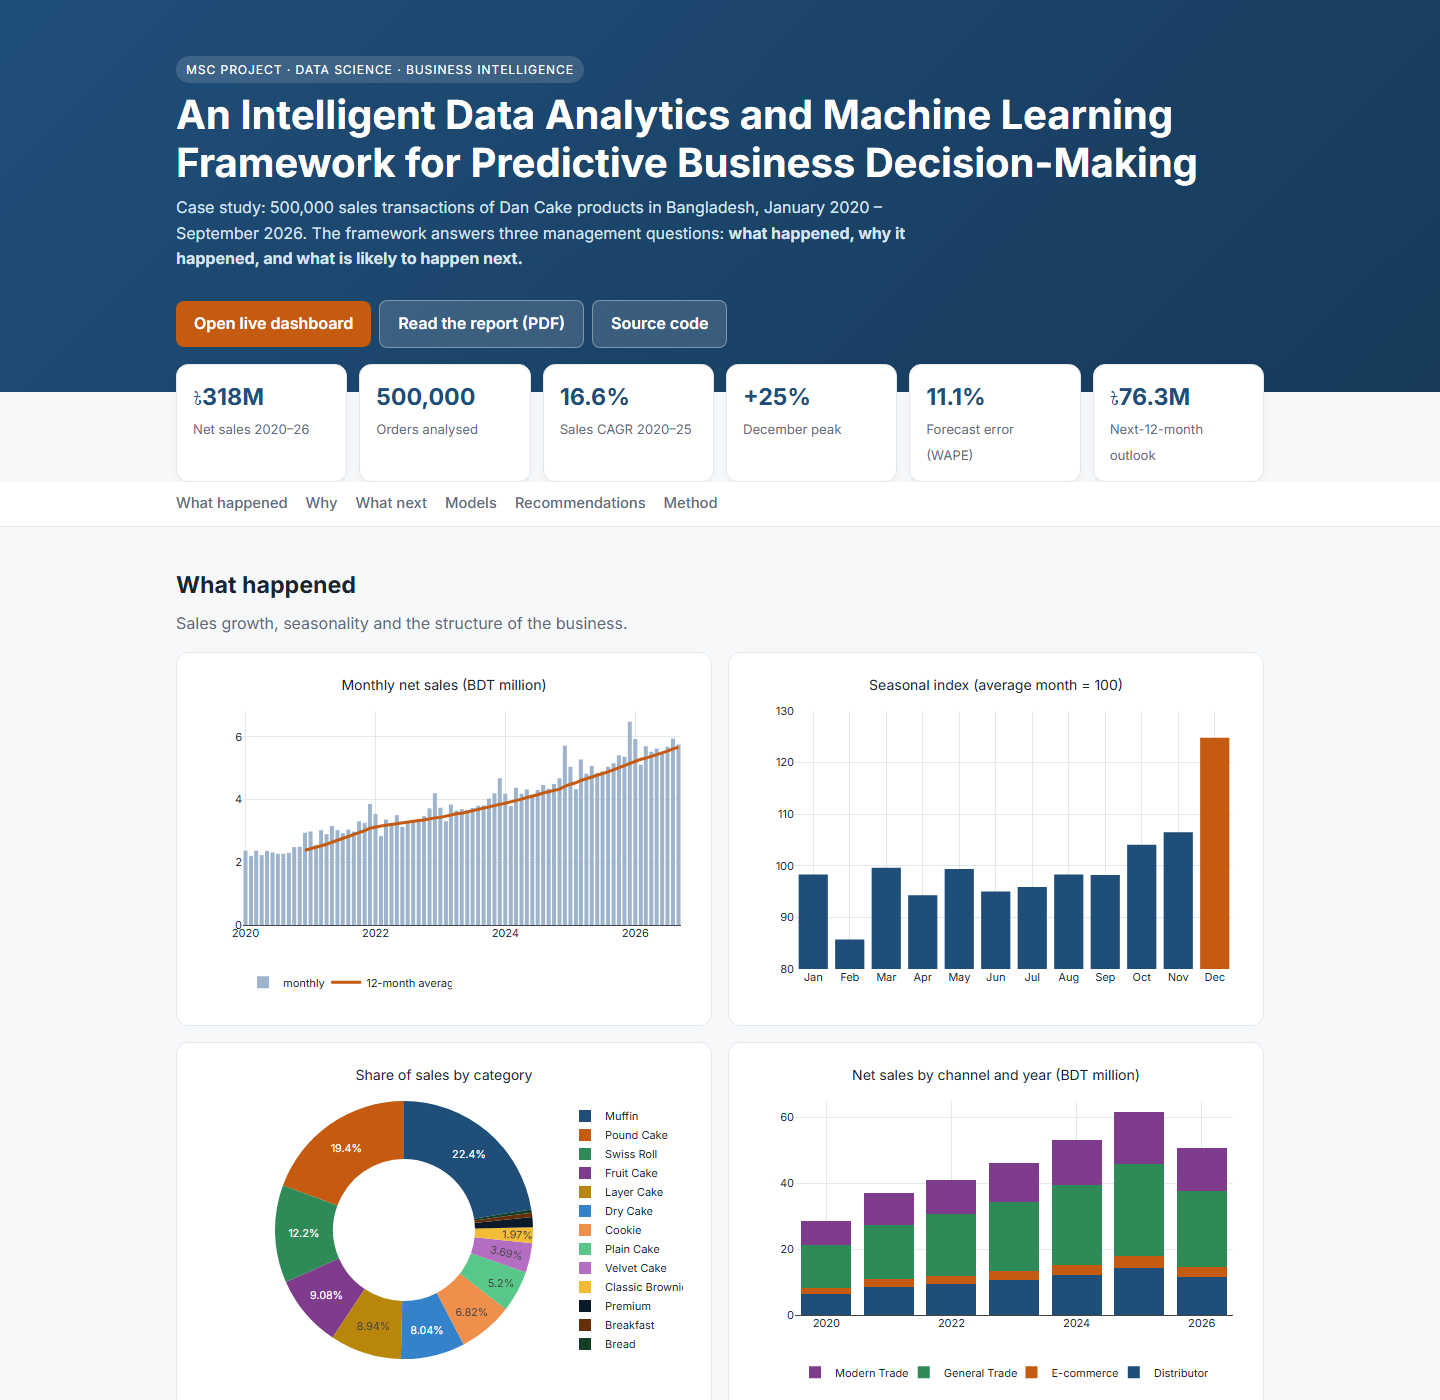
\includegraphics[width=\linewidth]{screens/website}
\caption{Project website on GitHub Pages, with links to the live dashboard, the report and the source code}\label{fig:website}
\end{figure}

\begin{figure}[htbp]\centering
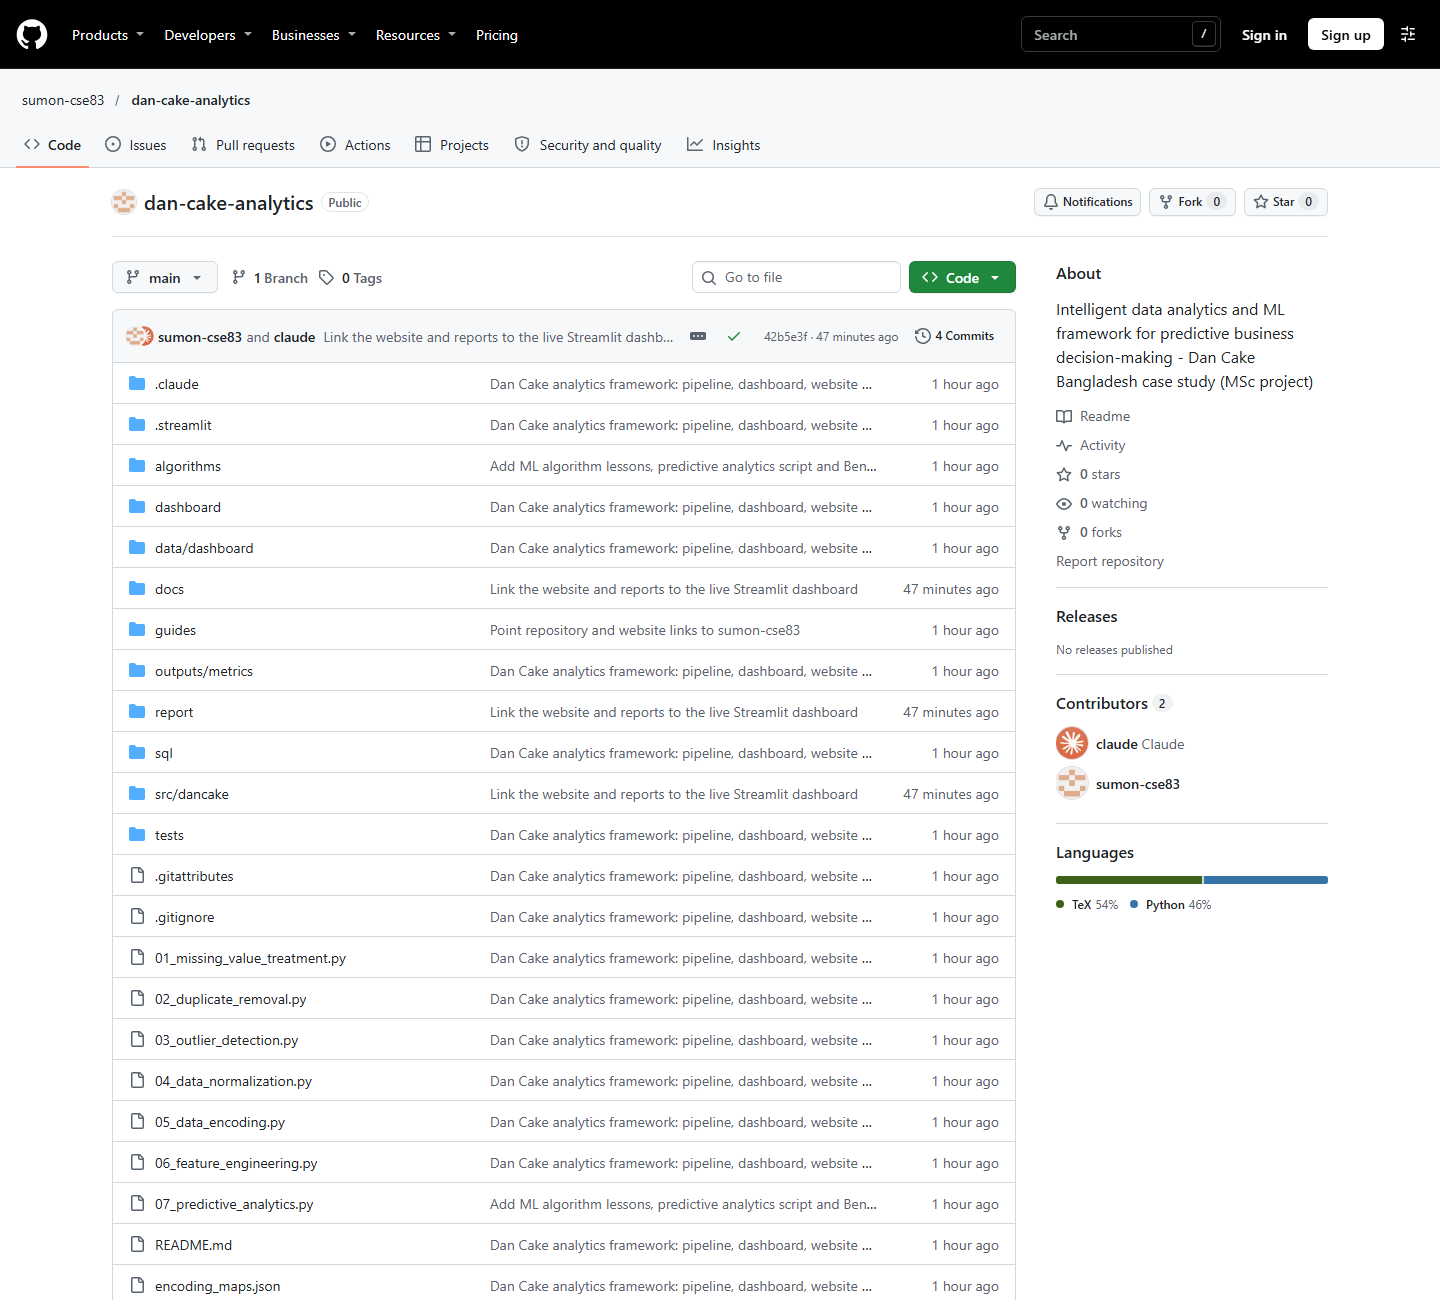
\includegraphics[width=\linewidth]{screens/github_repo}
\caption{Public GitHub repository holding the code, the dashboard data, the website and the report}\label{fig:github}
\end{figure}

If a custom domain name is bought later, it can be attached to GitHub Pages through a DNS \texttt{CNAME} record
without any change to the code. \Cref{app:reproduce} gives the step-by-step deployment procedure.

\section{Decision-support layer}
The final layer turns model outputs into recommendations. The module \texttt{insights.py} reads the metric
files and fills sentence templates with the current results. Every insight therefore stays up to date when new
data are processed, and none is typed by hand. The insights generated for this dataset are:

\begin{enumerate}[leftmargin=*,itemsep=4pt]
\item \textbf{Growth (What happened).} Net sales grew from 2020 to 2025 at 16.6\% a year, but units grew only 5.0\% a year; on average 11.3 percentage points of annual growth came from higher prices and mix, 5.0 from volume. \emph{Recommendation:} Track volume growth as a separate KPI; price-led growth is not sustainable indefinitely.
\item \textbf{Pricing (Why it happened).} After controlling for product, year and season, the estimated price elasticity of demand is +0.09 (95\% CI -0.28 to +0.46), i.e. not significantly different from zero. Discounts show no relationship with order size (Spearman rho = 0.001). \emph{Recommendation:} Review the discount budget (BDT 7.7 million over the period): discounts do not appear to buy volume.
\item \textbf{Seasonality (What happened).} December is the peak month (index 125, average month = 100) and February the weakest (86). The seasonal effect is statistically strong (Kruskal-Wallis p < 0.001). \emph{Recommendation:} Build stock and distributor capacity from October; schedule promotions and maintenance in February.
\item \textbf{Portfolio (What happened).} Muffin is the largest category (22.4\% of sales); the top 10 of 52 products deliver 38.5\% of revenue and 27 products form the 'A' class (80\% of sales). \emph{Recommendation:} Protect availability of A-class products first; review C-class products for rationalisation or repositioning.
\item \textbf{Portfolio (Segmentation).} Clustering finds 5 product segments; 'Premium \& gift packs' grows fastest (+7.8\% units a year, 33.3\% of sales). \emph{Recommendation:} Prioritise shelf space and marketing for 'Premium \& gift packs'.
\item \textbf{Market (What happened).} Dhaka alone generates 43.9\% of sales and Dhaka plus Chattogram 58.3\%. General Trade is the largest channel (45.6\%), while E-commerce is 5.9\%. \emph{Recommendation:} Reduce concentration risk by developing secondary cities and scaling E-commerce, which grows from a small base.
\item \textbf{Market (Segmentation).} The 'Emerging high-growth cells' segment (19 region-channel-customer cells, mainly Cumilla, Khulna, Mymensingh) is growing at +33.2\% a year, the fastest of the 4 market segments. \emph{Recommendation:} Allocate field-sales and digital-marketing effort to these emerging cells.
\item \textbf{Orders (Prediction).} Whether an order will be large ($\geq$ 10 units) is moderately predictable (best ROC-AUC 0.712, Logistic Regression); channel is by far the strongest driver: 48\% of distributor orders are large versus 8\% online. \emph{Recommendation:} Use the large-order score for delivery-vehicle and stock allocation, mainly at channel level.
\item \textbf{Forecast (What will happen).} The Support Vector Regression model forecasts next month's product demand with 11.1\% weighted error, 24\% lower RMSE than the seasonal-naive rule. Net sales for 2026-10 to 2027-09 are forecast at BDT 76.3 million (+12.1\% on the previous 12 months; 80\% range BDT 72.7 million - BDT 79.9 million). \emph{Recommendation:} Use the product-level forecast for the monthly production plan and the interval for safety stock.
\item \textbf{Risk (Anomalies).} 28 of 2,465 trading days were flagged as unusual. In a controlled test, rules plus Isolation Forest caught 91\% of 1,000 planted data errors. \emph{Recommendation:} Run the anomaly screen daily and investigate flagged days and orders before month-end reporting.
\end{enumerate}

Each insight is tagged by area and by the management question it answers. Each is paired with a concrete
action, so the dashboard serves as a \emph{decision-support system}, not merely a reporting tool.

\section{System evaluation}
The proposal asked for the system to be evaluated on predictive performance, usability, analytical usefulness,
visualisation quality and processing efficiency. \Cref{tab:syseval} summarises the evidence.

\begin{table}[htbp]\centering\small
\caption{Evaluation of the framework against the criteria in the proposal}\label{tab:syseval}
\begin{tabularx}{\linewidth}{@{}lX@{}}
\toprule
\textbf{Criterion} & \textbf{Evidence} \\ \midrule
Predictive performance & All ML forecasters beat naive baselines; best WAPE \BestRegWAPE\%; company-level MAPE \HWMAPE\%; classification ROC-AUC \ClsAUC (\cref{ch:models}); confirmed independently by the algorithm study (\cref{ch:algorithms}) \\
Analytical usefulness & Insights on growth quality, discount ineffectiveness, seasonality, concentration risk, segments and anomalies, each with a recommended action \\
Usability & One set of global filters; nine task-oriented pages with bookmarkable addresses; plain-language captions; downloadable forecasts; runs in any browser without installation \\
Visualisation quality & Principles of Few, Tufte and Knaflic: KPI cards, sorted bars, heat maps, intervals on forecasts, no 3-D or decorative charts, consistent palette \\
Processing efficiency & Data validation and cleaning of \NRows rows in under 20 seconds; warehouse load in \WarehouseSeconds s; full pipeline including model tuning in about 20 minutes on a standard laptop; dashboard data about 2 MB \\
Availability & Publicly deployed on free HTTPS platforms with automatic redeployment on every push (\cref{sec:deployment}) \\
Reproducibility & One command regenerates all data, models, figures, tables and numbers; fixed random seed; automated tests; version history on GitHub \\ \bottomrule
\end{tabularx}
\end{table}

A formal usability study with managers was beyond the time available. It is recommended as future work: a short
task-based test with a System Usability Scale questionnaire would complete the evaluation.
